\chapter{Project milestones}

What follows are milestones for the project development.
Achieving each one is a step closer to the end goal of a functioning documentation-generating tool.

Said milestones are based on the analysis of current documentation tools (see \ref{sec:whatisavailable}), developer needs (see \ref{sec:whatdouserswant}), personal experience, and general project development guidelines.

\section{Proof of concept}

Creating a proof of concept program will help understand whether the project is realistic, what challenges will occur and how to overcome them.
The main drawback of this is that it will take additional time; however, the gained perspectives are quintessential for the correct planning of the project.

The main focus of this milestone is to find out how to extract the necessary data for documentation generation and attempt to generate said documentation.
All other requirements based on the takeaways from the survey (see \ref{ssec:questionnaireeval}) can be omitted from this stage, as they have been proven via other personal projects or are publicly available for reference.

\section{Evaluations and project planning}

Concise planning of the project, based on the gained experience from the proof of concept, will, as a result, yield a higher quality product.
Extensibility will be the key feature of the project. Careful planning of the code structure is required to avoid unnecessary complications.
Meanwhile, the planning phase shouldn't take unreasonable effort, as the ratio of time spent to results will diminish over time (as seen in \ref{fig:overplanning}). \cite{ruparelia_stop_2016}

\begin{figure}[H]
    \centering
    \caption{Overplanning visualized}
    \label{fig:overplanning}
    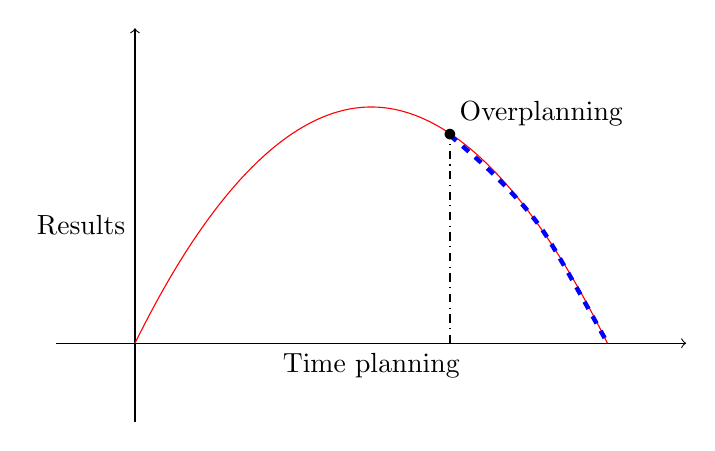
\begin{tikzpicture}
        \draw [->] (-4, 0)--(4,0) node [midway, below]{Time planning};
        \draw [->] (-3, -1)--(-3,4) node[left, midway]{Results};

        \draw [red] (0, 3) parabola(-3,0); % Left
        \draw [red] (0, 3) parabola(3,0); % Right
        \draw [ultra thick, blue, dashed] plot [smooth] coordinates {(1, 2.64) (1.6,2.1) (2.2, 1.40) (3, 0)}; % Right

        \draw [dash dot] (1,0)--(1, 2.64);

        \draw (1, 2.64) node [above right]{Overplanning};
        \draw (1, 2.64) node {$\bullet$};
    \end{tikzpicture}
\end{figure}

\section{Basic structure}
